\section{Results}
\label{sec:results}

Over half a million cosmic muon events are recorded. To study the TP efficiency, we reconstruct tracks from clusters of MMFE8 hits. The BCID of these hits is required to be in a 15 BC window around the scintillator trigger. We require that a good MMFE8 track with at least 3 X boards and 3 U,V boards be reconstructed. We apply a fiducial cut of (0, 170 mm) in the x-coordinate due to the aforementioned implementation limitations. We then ask, given an MMFE8 candidate event, if there was a corresponding TP track. 
\par Because the distribution of cosmic muons follows the well-known $\cos^2 \theta$ distribution, to extract the efficiency for perpendicular tracks we plot the efficiency as a function of the MM track angle. We see a plateau in this distribution (Fig. \ref{fig:data}) at 94\% for MM tracks with small angles. To estimate the contribution of delta rays to the efficiency loss, we make a requirement of one or fewer MM clusters per board. This increases the efficiency to 96\%. 

\begin{figure}[!htpb]
  \begin{center}
    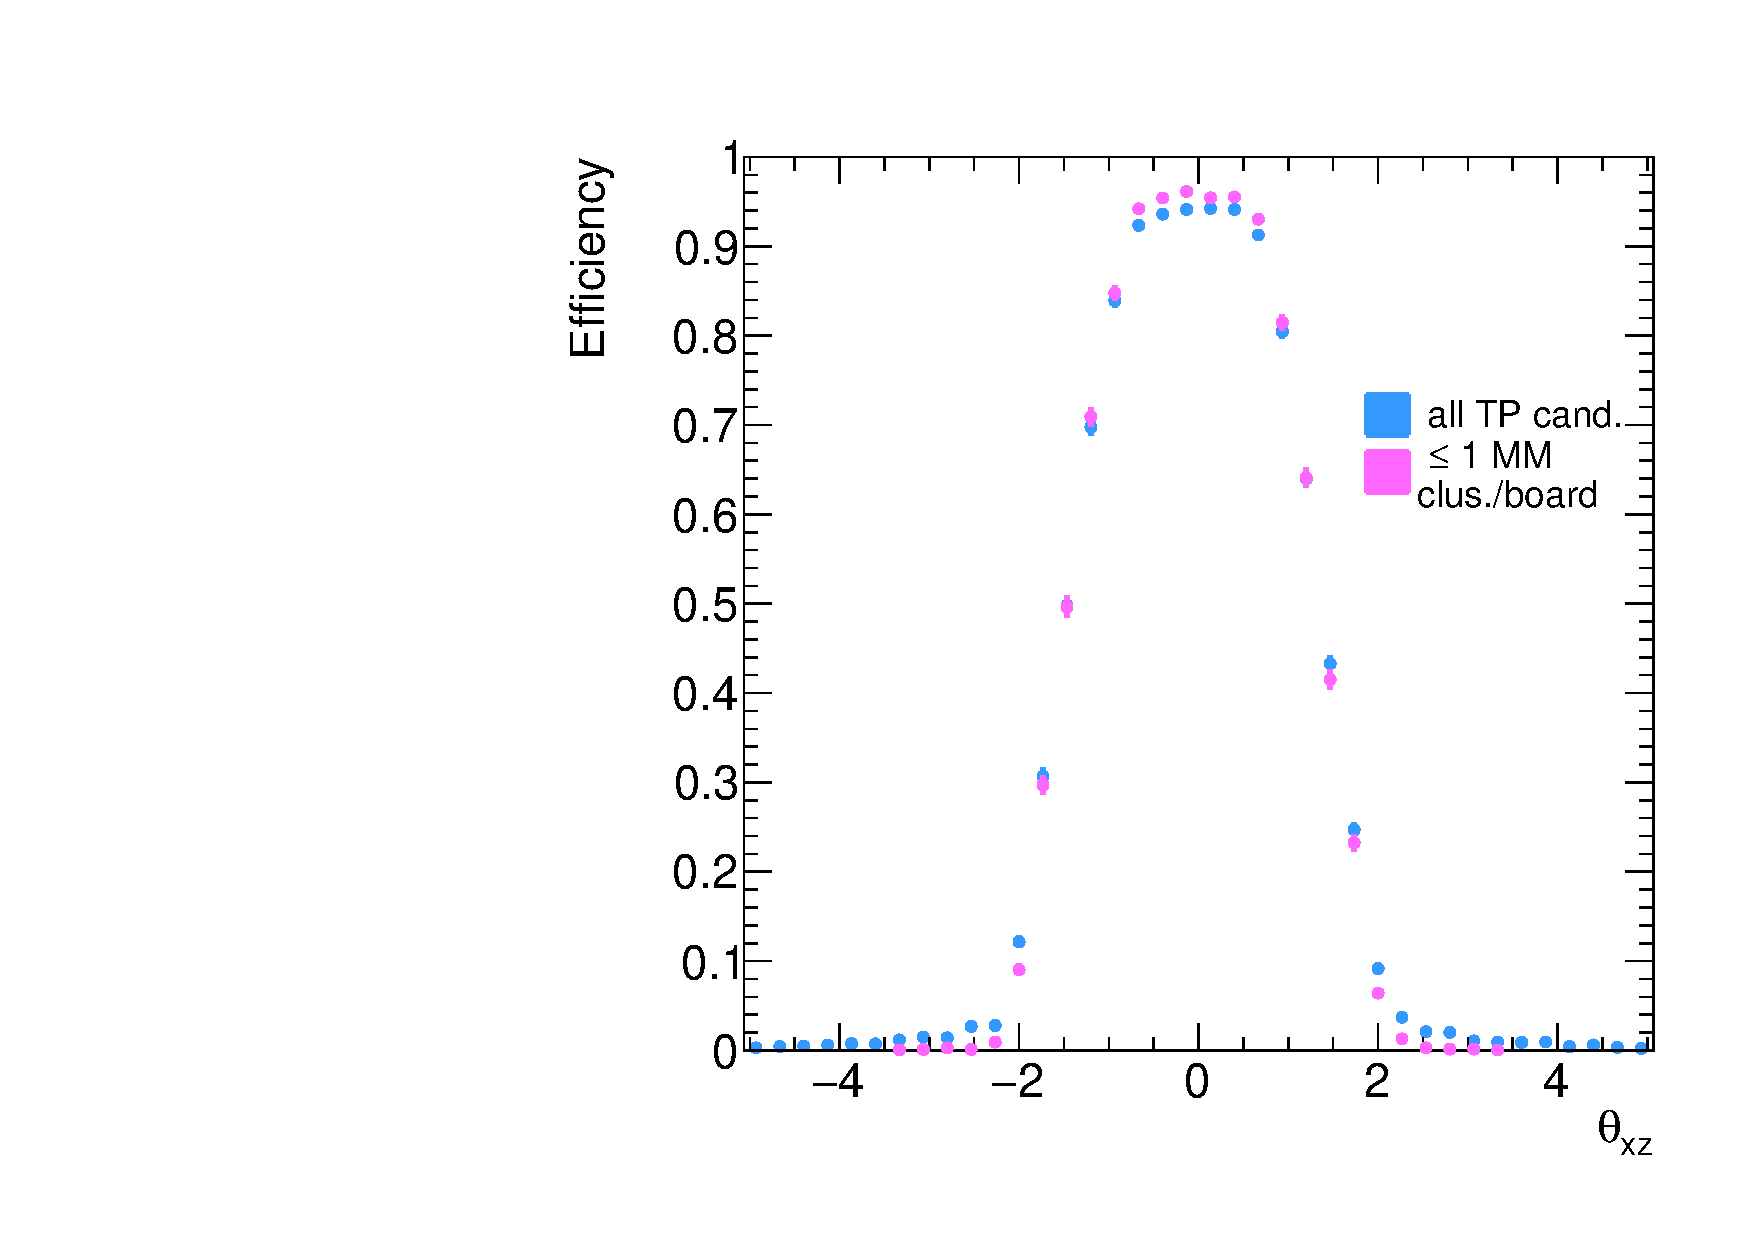
\includegraphics[width=0.48\textwidth]{figures/tpeff_vs_theta_zoom.pdf}
    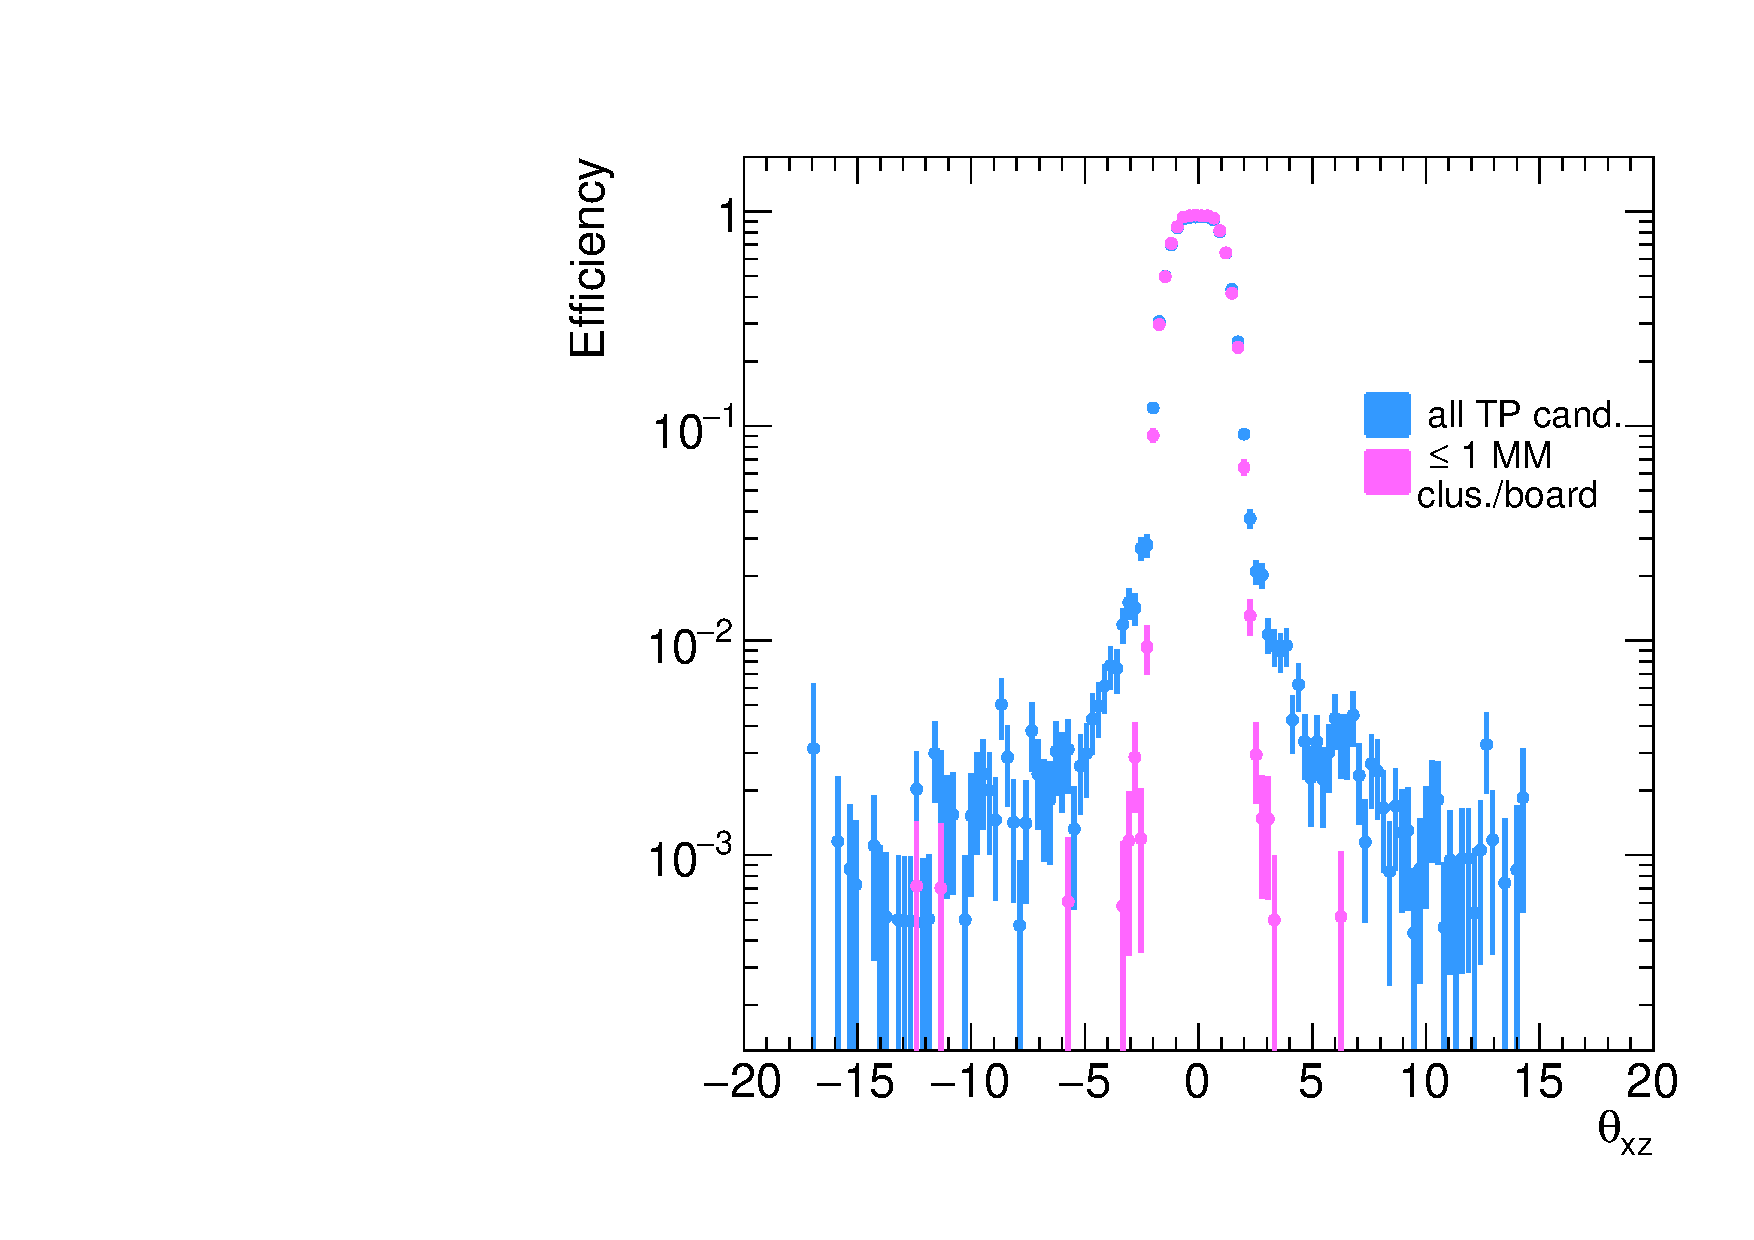
\includegraphics[width=0.48\textwidth]{figures/tpeff_vs_theta_log.pdf}
  \end{center}
  \vspace{-10pt}
  \caption{The efficiency of finding a TP track as a function of track angle from -5 to 5 degrees (left), and from -20 to 20 degrees (right). The efficiency is shown for all MM tracks that are triggerable and those which have one or fewer MM clusters per board.}
  \label{fig:data}
\end{figure}
\FloatBarrier

\par To understand the reason for the 4\% efficiency loss, we point to the effect of the non-Gaussianity of the ART position resolution. The 12-strip road size, motivated in Ref. \cite{tpsim}, assumes that the ART spatial resolution has a $\sigma$ of 1 strip. This assumption was motivated by the data in Ref. \cite{mmtp}, but failed to take into account the effect of non-Gaussian tails. We study the effect of using a functional form of the ART residuals, shown in Fig. \ref{fig:smear}, in simulation using HOTPOT. We see that for 8-cluster tracks, we see about a 1\% loss, but for 7-cluster tracks, we see an 8\% loss. The final impact of the ART residual tails in the NSW is dependent on the efficiency of the Micromegas chambers and front-end electronics. Sigh.
\begin{figure}[!htpb]
  \begin{center}
    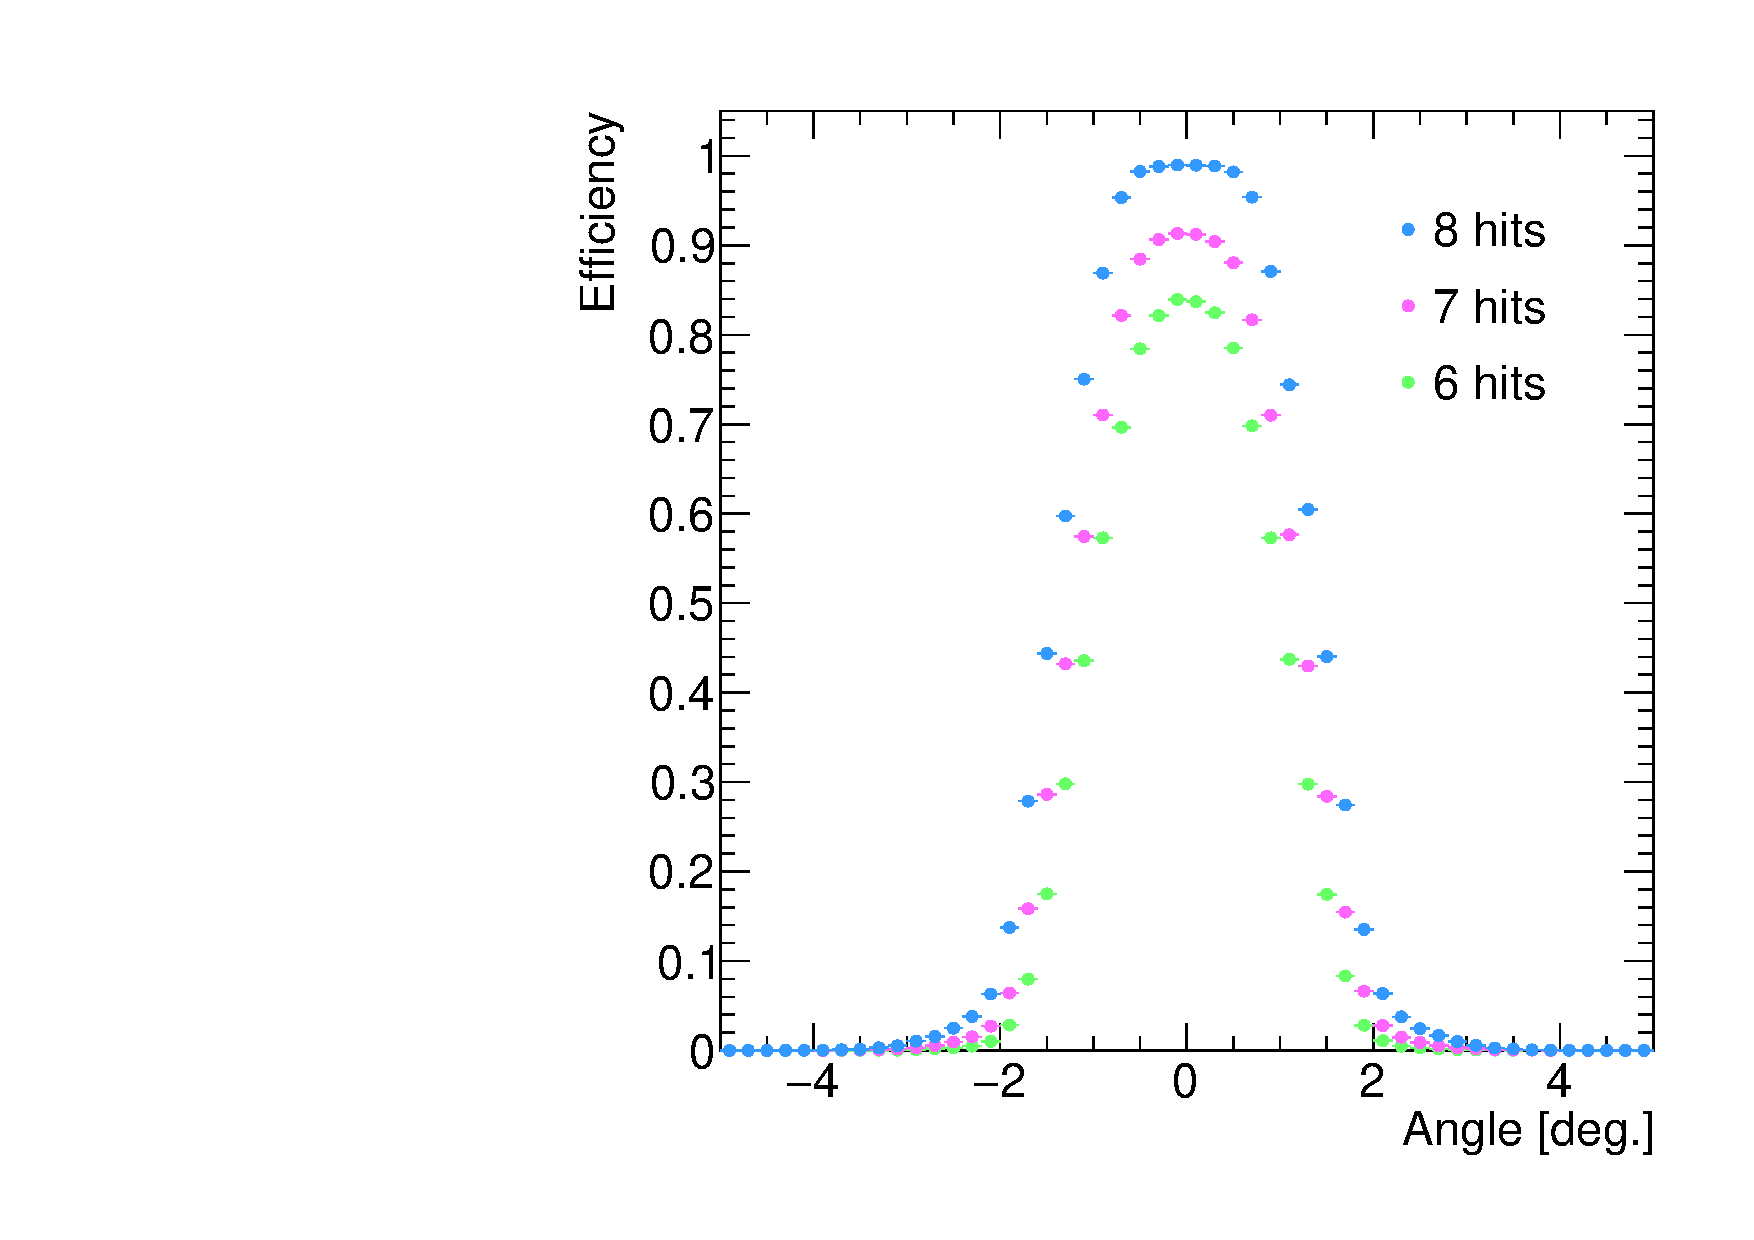
\includegraphics[width=0.48\textwidth]{figures/sim_eff_nhits_lin.pdf}
    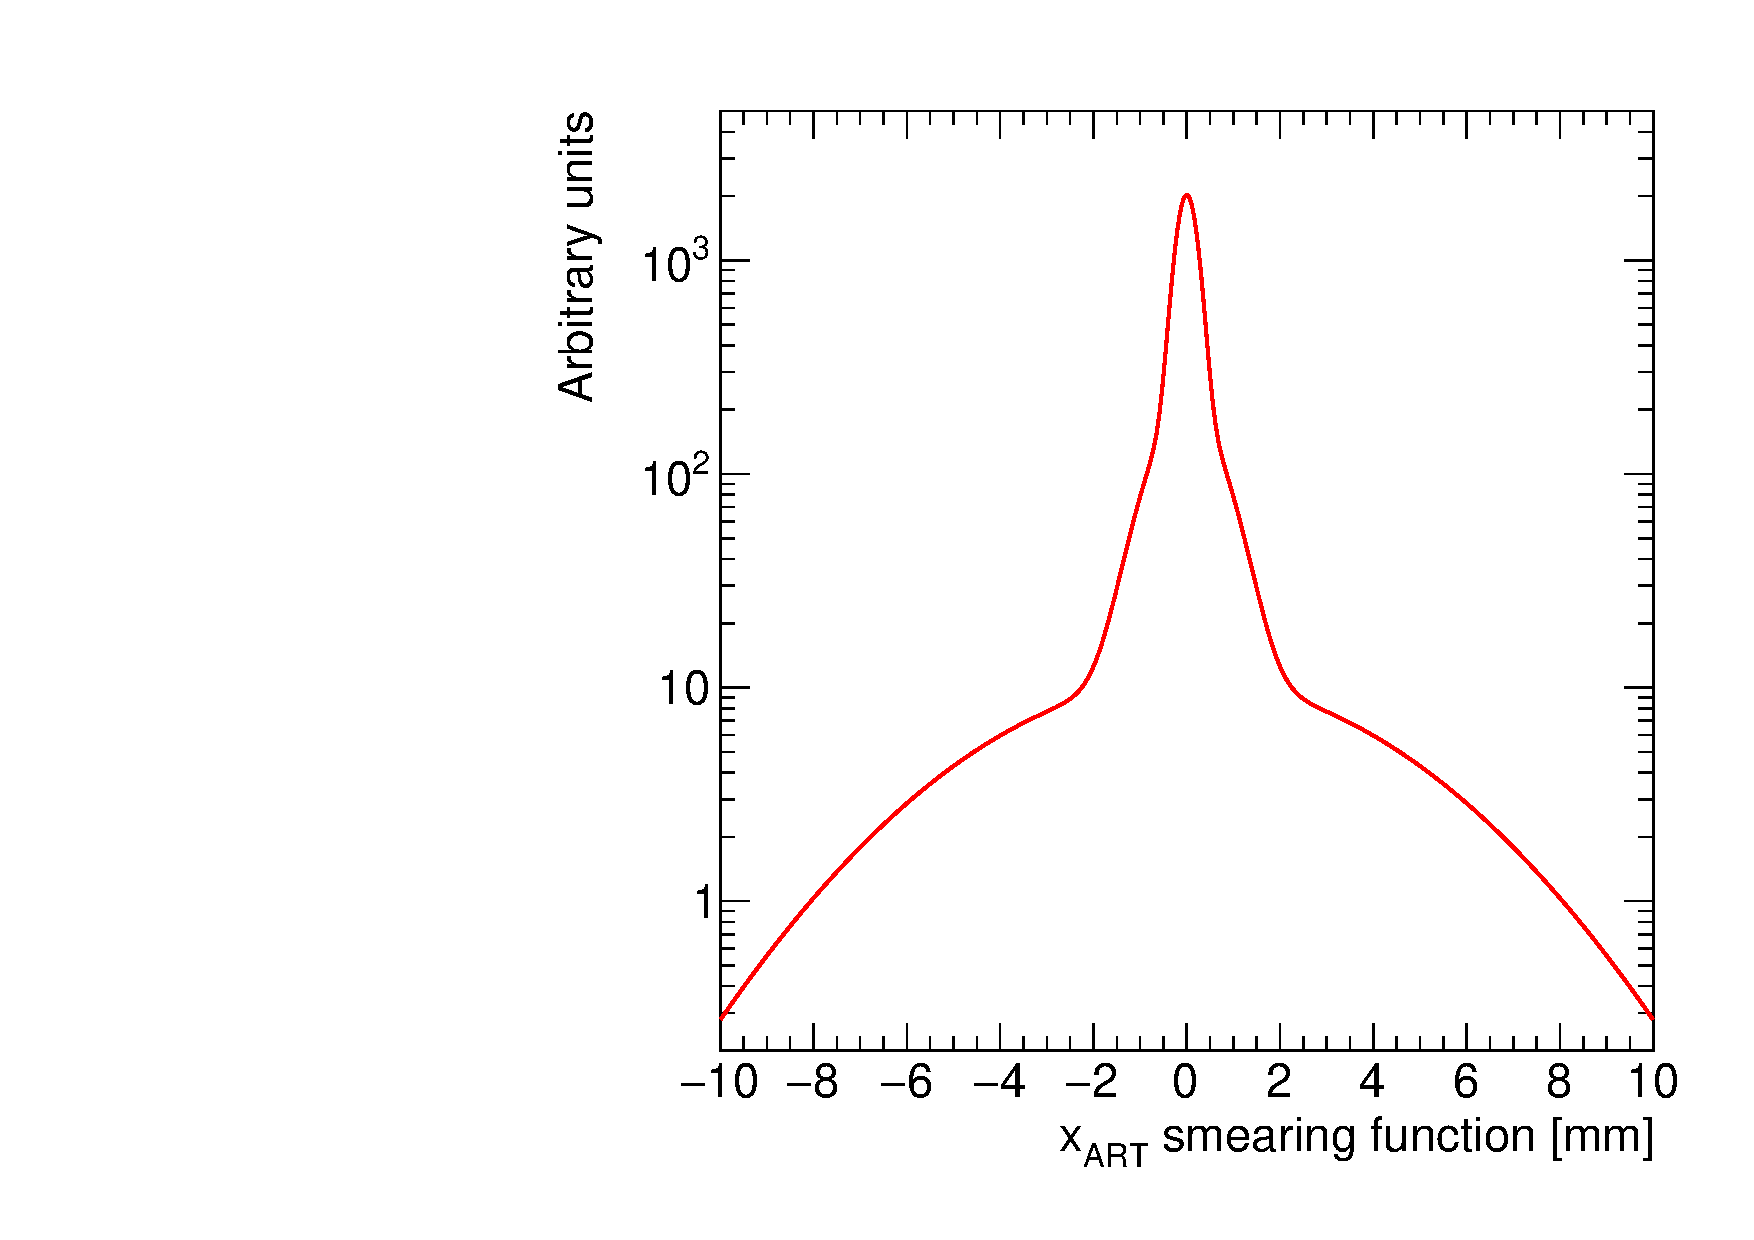
\includegraphics[width=0.48\textwidth]{figures/smear.pdf}
  \end{center}
  \vspace{-10pt}
  \caption{The efficiency of finding a TP track as a function of track angle in simulation (left). The distribution is plotted assuming 6, 7, and 8 hits in a track. The ART hits are smeared with a data-derived ART position-smearing function (right). This function is derived from data.}
  \label{fig:smear}
\end{figure}
